\chapter{Maquette de l'interface homme-machine}

\section{Connection}
Au lancement de l'application l'utilisateur doit pouvoir procéder à toutes les
étapes de la méthode GTD. Cependant, la connexion est indispensable à chacune
des étapes suivantes. En effet, les données sont stockées dans un compte
distant identifié par un login et protégé par un mot de passe. L'interface
suivante permet donc de se connecter, s'inscrire et renvoyer son mot de passe
en cas de perte de celui-ci.

\begin{figure}[H]
  \begin{center}
  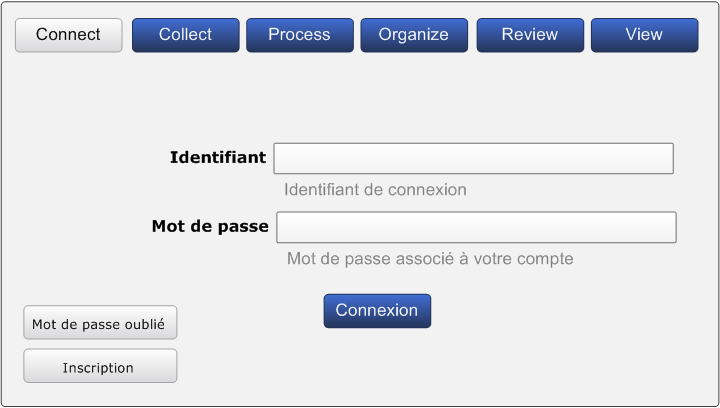
\includegraphics[scale=0.5]{livrable2/images/connect.png}
  \caption{Mockup - Connection}
  \end{center}
\end{figure}

Une fois que l'utilisateur est connecté, il peut effectuer l'ensemble des
étapes de la méthode GTD ou seulement celle qui l'intéresse. L'utilisateur doit
en effet être libre de choisir ce qu'il veux faire au moment où il lance
l'application. Il peut donc le faire par le menu présent en haut de
l'interface, présentant dans l'ordre chronologique les différentes étapes.

\section{Collect}
Après avoir cliqué sur l'onglet Collect, l'utilisateur dispose d'une interface offrant
les fonctionnalités d'un pense-bête. En effet, Collect est une réflexion de
l'utilisateur. La seule aide que pour fournir l'application est un stockage des
idées n'ayant pas eu le temps d'être traité dans Process. Il peut donc ajouter (bouton +) et supprimer (bouton -) simplement des idées, ici sous forme de
post-it.


\begin{figure}[H]
  \begin{center}
  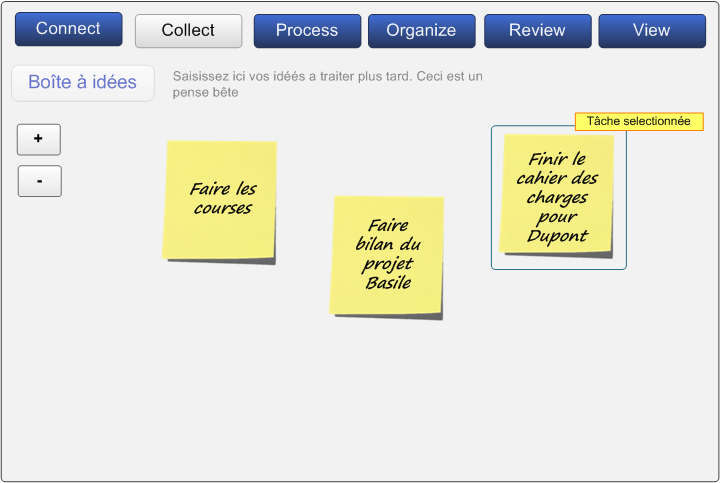
\includegraphics[scale=0.5]{livrable2/images/collect.png}
  \caption{Mockup - Collect}
  \end{center}
\end{figure}

\section{Process}
Lorsque l'utilisateur clique sur process, il dispose d'une interface affichant
les idées qu'il a actuellement dans son pense-bête et d'une interface de saisie
de tâches. Il peut donc aisément créer ses tâches avec toutes les informations
nécessaires sans oublier celles qui sont dans son pense-bête.


\begin{figure}[H]
  \begin{center}
  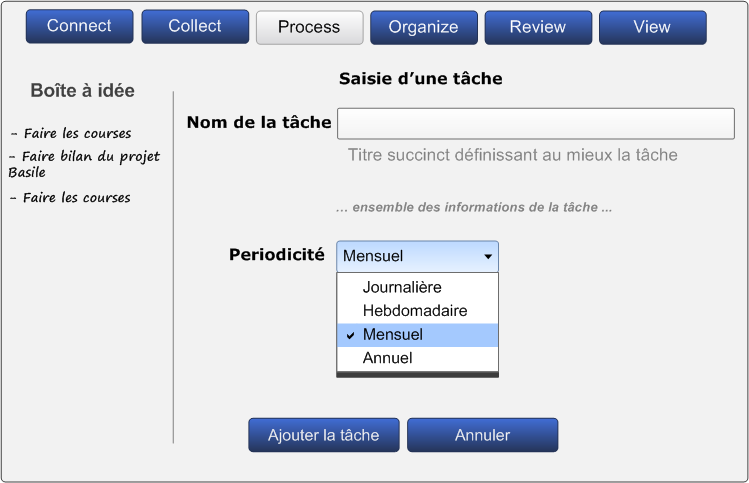
\includegraphics[scale=0.5]{livrable2/images/process.png}
  \caption{Mockup - Process}
  \end{center}
\end{figure}


\section{Organize}
Lorsque l'utilisateur clique sur organize, il dispose de deux fonctionnalités :
\begin{itemize}
  \item Organiser les tâches en projet,
  \item Déléguer une tâche.
\end{itemize}
L'organisation inclut la création de projet (bouton +), la définition du
contexte par défaut du projet, ainsi que l'ajout des tâches dans un projet par
glisser-déposer de la liste 'tâches disponibles' vers 'tâches affectées au
projet', en définissant un ordre chronologique.
Pour la délégation il suffit de sélectionner une tâche, puis une personne à qui
déléguer, et enfin de valider.

\begin{figure}[H]
  \begin{center}
  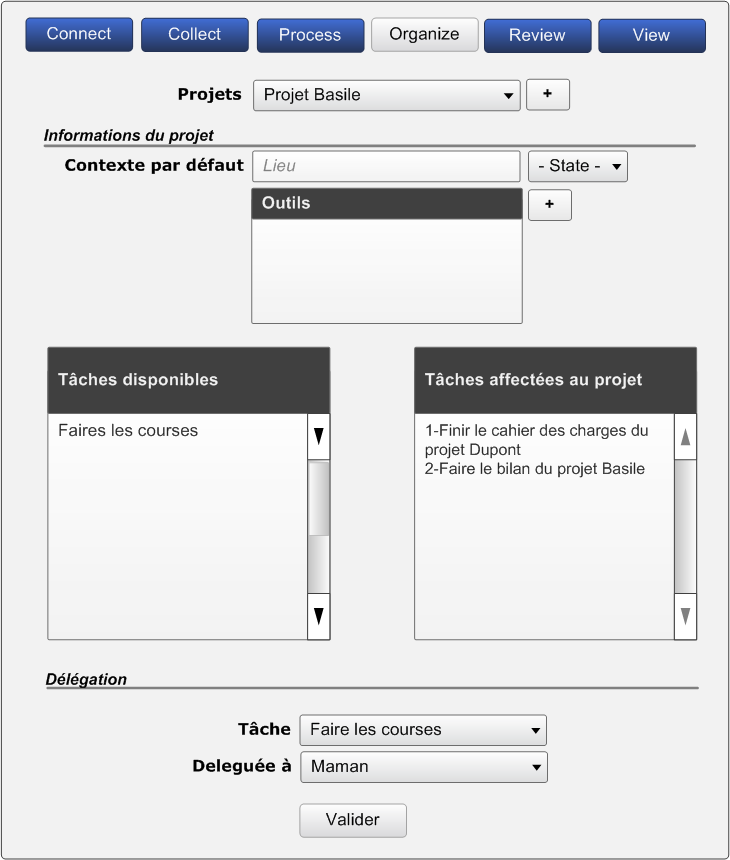
\includegraphics[scale=0.5]{livrable2/images/organize.png}
  \caption{Mockup - Process}
  \end{center}
\end{figure}

\section{Review}
L'interface Review permet simplement de mettre à jour les informations de
certaines tâches. Elle correspond donc à l'interface de process.

\begin{figure}[H]
  \begin{center}
  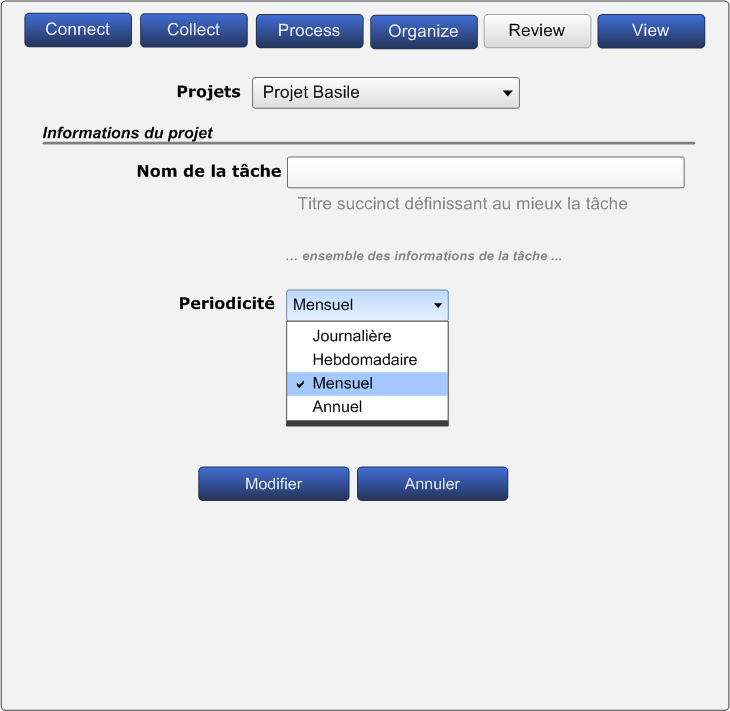
\includegraphics[scale=0.5]{livrable2/images/review.png}
  \caption{Mockup - Review}
  \end{center}
\end{figure}

\section{View}
La vue est l'opération finale, elle permet d'afficher les tâches en agenda ou
en écheancier afin de conseiller l'utilisateur dans la bonne gestion de son
temps. Le calendrier affiche les jours occupés et la liste des tâches présentes
dans l'ordre de leur priorité depuis la date selectionnée dans le
calendrier.

\begin{figure}[H]
  \begin{center}
  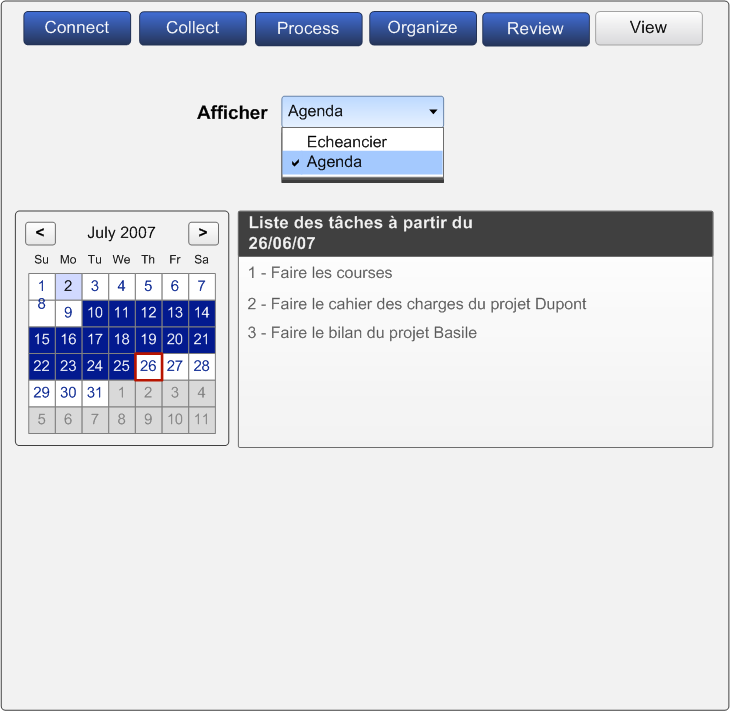
\includegraphics[scale=0.5]{livrable2/images/view.png}
  \caption{Mockup - View}
  \end{center}
\end{figure}